
\chapter{Reinforcement Learning}

\acrfull{rl} is a field of Machine Learning that is experiencing a period of great fervour in the world of research, fomented by recent progress in \acrfull{dl}. This event opened the doors to function approximation with \acrfull{nn} and \acrfull{cnn} developing what is nowadays known as Deep Reinforcement Learning.

\acrshort{rl} represents the third paradigm of Machine Learning alongside supervised and unsupervised learning. The idea behind  this research field is that the learning process to solve a decision-making problem consists in a sequence of trial and error where the \textit{agent}, the protagonist of \acrshort{rl}, could discover and discriminate valuable decisions from penalising ones exploiting information given by a \textit{reward signal}. This interaction has a strong correlation with what human beings and animals do in the real world to forge their behaviour.

Recently \acrshort{rl} has known a remarkable development and interests in video games: it managed to beat world champions at the game of Go \cite{silver2016mastering} and Dota with superhuman results and to master numerous Atari video games \cite{mnih2013playing} from raw pixels. Decisions, actions and consequences make video games a simulated reality on which to exploit and test the power of \acrshort{rl} algorithms.
It is essential to realise that the heart of \acrshort{rl} is the science of decision making. This fact makes it compelling and general for many research fields ranging from Engineering, Computer Science, Mathematics, Economics, to Psychology and Neuroscience.

Before discussing the results of this thesis, it is good to clarify everything that today represents the state-of-the-art in order to understand the universe behind this new paradigm better. Indeed, the exploration of this field of research is the main aim of this chapter: the first section begins with the definition of the notation used and with the theoretical foundations behind \acrshort{rl}, then in the second section it moves  progressively towards what is Deep \acrshort{rl} through a careful discussion of the most essential algorithms paying more attention to those used during the thesis project.

The elaboration of this chapter is inspired by \cite{silver2015lectures}, \cite{sutton2018reinforcement}, \cite{openai2018spinningup}, \cite{lapan2018deep} and \cite{franccois2018introduction}.

\section{Fundamentals of Reinforcement Learning} \label{fundreinflearn}

%\todomacaluso{
%	\begin{itemize}
%		\item Introduction
%		\item Central concepts regarding fundamentals (e.g. Agent, Environment, Reward, Return)
%		\item Markov Decision Process (MDP)
%		\item Model-based prevision and control: just a brief introduction to Dynamic Programming and Policy/Value Iteration
%		\item Model-free prevision and control: a brief introduction to Monte Carlo and TD Learning approaches (SARSA and Q-Learning)
%	\end{itemize}	
%}

Reinforcement Learning is a computational approach to Sequential Decision Making. It provides a framework that is exploitable with decision-making problems that are unsolvable with a single action and need a sequence of actions, a broader horizon, to be solved. 

This section aims to present the fundamental ideas and notions behind this research field in order to help the reader to develop a baseline useful to approach \vref{deepreinflearn} about Deep Reinforcement Learning.

\subsection{The Reinforcement Learning Problem}

The primary purpose of \acrshort{rl} algorithms is to learn how to improve and maximise a future reward by relying on interactions between two main components: the agent and the environment. 

The \textit{agent} is the entity that interacts with the environment by making decisions based on what it can observe from the state of the surrounding situation. The decisions taken by the agent consist of \textit{actions} ($a_t$).  The agent has no control over the environment, but actions are the only means by which it can modify and influence the environment.

Usually, the agent has a set of actions it can take, which is called \textit{action space}.
Some environments have discrete action spaces, where only a finite number of moves are available (e.g. $\mathcal{A} = [\text{North}, \text{South}, \text{East}, \text{West}]$ choosing the direction to take in a bidimensional maze). On the other side, there are continuous action spaces where actions are vectors of real values.
This distinction is fundamental to choose the right algorithm to use because not all of them could be compatible with both types: according to the needs of the specific case, it may be necessary to modify the algorithm to make it compatible.

The \textit{environment} represents all the things that are outside the agent. At every action received by the agent, it emits a reward, an essential aspect of \acrshort{rl}, and an observation of the environment.

The \textit{reward} $r_t$ is a scalar feedback signal that defines the objective of the \acrshort{rl} problem. This signal allows the agent to be able to distinguish positive actions from negative ones in order to reinforce and improve its behaviour. It is crucial to notice that the reward is local: it describes only the value of the latest action. Furthermore, actions may have long term consequences, delaying the reward. As it happens with human beings' decisions, receiving a conspicuous reward at a specific time step does not exclude the possibility to receive a small reward immediately afterwards and sometimes it may be better to sacrifice immediate reward to gain more rewards later.


In this context, many features make \acrshort{rl} different from supervised and unsupervised learning.
Firstly, there is no supervisor: when the agent has to decide what action to take, there is no entity that can tell him what the optimal decision is in that specific moment. The agent receives only a reward signal which may delay compared to the moment in which it has to perform the next action. 
This fact brings out another significant difference: the importance of time. The sequentiality links all actions taken by the agent, making resulting data no more \acrfull{iid}.

Given these definitions, it is noticeable that the primary purpose of the agent is to maximise the cumulative reward called \textit{return}.

The \textit{return $g_t$} is the total discounted reward starting from timestep $t$ defined by \vref{eq:return} where $\gamma$ is a \textit{discount factor}.

\begin{equation} \label{eq:return} 
	g_t = r_{t+1} + \gamma r_{t+2} + \dots = \sum_{k=0}^{\infty} \gamma^k r_{t+k+1}, \;\;\;\gamma \in [0,1)
\end{equation}

 Not only the fact that animal and human behaviour show a preference for immediate rewards rather than for the future ones motivates the presence of this factor, but it is also mathematically necessary: an infinite-horizon sum of rewards may not converge to a finite value. Indeed, the return function is a geometric series, so, if $\gamma \in [0,1)$, the series converges to a finite value equal to $1/(1-\gamma)$. For the same convergence sake, the case with $\gamma = 1$ makes sense only with a finite-horizon cumulative discounted reward.

The other data emitted by the environment is the \textit{observation} ($o_t$) that is related to the \textit{state} ($s_t$). It represents a summary of information that the agent uses to select the next action, while the \textit{state} is a function of the \textit{history} the sequence of observation, actions and rewards at timestep $t$ as shown in \vref{eq:history}.

\begin{equation}\label{eq:history}
h_t = o_1, r_1, a_1, \dots, a_{t-1}, o_{t}, r_t, \;\;\;\;\; s_t = f(h_t)
\end{equation}

The sequence of states and actions is named \textit{trajectory} ($\tau$): it is helpful to represent an episode in \acrfull{rl} framework.

The state described above is also called \textit{agent state} $s_t^a$, while the private state of the environment is called \textit{environment state} $s_t^e$. This distinction is useful for distinguishing fully observable environments where $o_t = s_t^e = s_t^a$, from partially observable environments where $s_t^e \neq s_t^a$.
In the first case, the agent can observe the environment state directly, while in the second one, it has access to partial information about the state of the environment.

Beyond the fact that this chapter will focus on fully observable environments, the distinction between state and observation is often unclear and, conventionally, the input of the agent is composed by the reward and the state as shown in \vref{fig:interactionsAE}.


\begin{figure}
	\centering
	\begin{tikzpicture}
	% node Agent
	\node[punkt] (agent) {Agent};
	% node Environment
	\node[punkt, below=2cm of agent] (env) {Environment};
	% node a_t
	\node[mylabel, below right=0.75cm and 0cm of agent] (action) {$a_t$};
	% node s_t
	\node[mylabel, below left=0.75cm and 0.8cm of agent] (state) {$s_t$};
	% node r_t
	\node[mylabel, below left=0.75cm and -0.3cm of agent] (reward) {$r_t$};
	% node s_t+1
	\node[mylabel, above left=-1.3cm and -1cm of env] (state) {$s_{t+1}$};
	% node r_t+1
	\node[mylabel,above left=-.3cm and -1cm of env] (reward1) {$r_{t+1}$};
	
	
	
	\draw[pil]   (agent.east) -- ($(agent.east) + (1.2cm,0cm)$)  |-  (env.east);
	\draw[pil]   ($(env.west) + (0,-0.2cm)$) -- ($(env.west) + (-1.2cm,-0.2cm)$);
	\draw[pil]   ($(env.west) + (-1.2cm,-0.2cm)$) -- ($(env.west) + (-2cm,-0.2cm)$) |-($(agent.west) + (0,0.2cm)$);
	\draw[pil]   ($(env.west) + (0,+0.2cm)$) -- ($(env.west) + (-1.2cm,+0.2cm)$);
	\draw[pil]   ($(env.west) + (-1.2cm,+0.2cm)$) -- ($(env.west) + (-1.6cm,+0.2cm)$) |-($(agent.west) + (0,-0.2cm)$);
	\draw[dashed]  ($(env.west) - (1.2cm,-0.5cm)$) -- ($(env.west) - (1.2cm,0.5cm)$);
	\end{tikzpicture}
	\caption[Interaction loop between Agent and Environment]{Interaction loop between Agent and Environment. The reward and the state resulting from taking an action become the input of the next iteration.}
	\label{fig:interactionsAE}
\end{figure}

Furthermore, a state is called \textit{informational state} (or \textit{Markov state}) when it contains all data and information about its history. Formally, a state is a Markov state if and only if satisfies \vref{eq:markov_state}.

\begin{equation} \label{eq:markov_state}
	\mathbb{P}[s_{t+1}| s_t] = \mathbb{P}[s_{t+1} | s_1, \dots, s_t]
\end{equation}

 It means that the state contains all data and information the agent needs to know to make decisions: the whole history is not useful anymore because it is inside the state. The environment state $s_t^e$ is a Markov state.
 
 With all the definitions shown so far, it is possible to formalise the type of problems on which \acrshort{rl} can unleash all its features: the \acrfull{mdp}, a mathematic framework to model decision processes. Its main application fields are optimization and dynamic programming.
 
 An \acrshort{mdp} is defined by 
 \begin{equation}\label{eq:mdp}
 \begin{gathered} 
 <\mathcal{S}, \mathcal{A}, \mathcal{P}, \mathcal{R}, \gamma>\\
 \begin{aligned}
 	\text{where}\hspace{10pt} \mathcal{S} & \text{ is a finite set of states} \\
 	\mathcal{A} & \text{ a finite set of actions} \\
 	\mathcal{P} & \text{ a state transition probability matrix}\;\;
 	 \mathcal{P}_{ss'}^a = \mathbb{P}[s_{t+1}= s' | s_t = s, a_t = a]\\
 	\mathcal{R} & \text{ a reward function}
 	 	\;\; \mathcal{R}_{s}^a = \mathbb{E}[r_{t+1} | s_t = s, a_t = a] \\
 	 \gamma & \text{ a discount factor such that } \gamma \in [0,1]
 \end{aligned}
 \end{gathered}
 \end{equation}


The main goal of an \acrshort{mdp} is to select the best action to take, given a state, in order to collect the best reward. 

In this quick overview of the central unit of \acrshort{rl}, the components that may compose the agent, the brain of the \acrshort{rl} problem can not be missing: they are the \textit{model}, the \textit{policy} and the \textit{value function}.

A \textit{model} consist of information about the environment. These data must not be confused with the ones provided by \textit{states} and \textit{observations}: they make it possible to infer prior knowledge about the environment, influencing the behaviour of the agent.

A \textit{policy} is the core of \acrshort{rl} because it is the representation of the agent's behaviour. It is a function that describes the mapping from states to actions.  The \textit{policy} is represented by $\pi$ and it may be deterministic  $a_t = \pi(s_t)$  or stochastic $\pi(a_t|s_t) = \mathbb{P}[a_t | s_t]$.

In this perspective, it is evident that the central goal of RL is to learn an optimal policy $\pi^*$. The optimal policy is a policy which can show to the agent what the most profitable way to achieve the maximum return is, what is the best action to do in a specific situation. In order to learn the nature of the optimal policy, \acrshort{rl} exploits value functions.

A \textit{value function} represents what is the expected reward that the agent can presume to collect in the future, starting from the current state. The reward signal represents only a local value of the reward, while the value function provides a broader view of future rewards: it is a sort of prediction of rewards.

It is possible to delineate two main value functions: the \textit{state value} function and the \textit{action value} function.

\begin{itemize}
	\item The \textit{State Value Function} $V^\pi(s)$ is the expected return starting from the state $s$ and always acting according to policy $\pi$.
	\begin{equation} \label{eq:statevalue}
		V^\pi(s) = \mathbb{E}_{\tau \sim \pi}[g_t | s_0 = s]
	\end{equation}
	\item The \textit{Action Value Function} $Q^\pi(s)$ is the expected return starting from the state $s$, taking an action $a$ and then always acting according to policy $\pi$.
	\begin{equation} \label{eq:actionvalue}
	Q^\pi(s, a) = \mathbb{E}_{\tau \sim \pi}[g_t | s_0 = s, a_0 = a]
	\end{equation}
\end{itemize}


\subsection{Bellman Equations}

Both \vref{eq:statevalue,eq:actionvalue} satisfy recursive relationships between the value of a state and the values of its successor states. It is possible to see this property deriving \textit{Bellman equations} -- shown in \vref{eq:bellman} and demonstrated in \vref{appendix:bellmaneq} -- where $s_{t+1}\sim \mathit{E}$ means that the next state is sampled from the environment $E$ and $a_{t+1}\sim \pi$ shows that the policy $\pi$ determines the next action.
\begin{align} \label{eq:bellman}
	\begin{split}
V^\pi(s_t) &= \mathbb{E}_{a_t \sim \pi, s_{t+1} \sim E}[r(s_t, a_t) + \gamma V^\pi(s_{t+1})] \\
		&= \sum_{a \in \mathcal{A}}\pi(a|s)\sum_{s' \in \mathcal{S}, r \in \mathcal{R}}P(s', r | s, a)\big[r + \gamma V^\pi(s')\big]\\
Q^\pi(s_t,a_t) &= \mathbb{E}_{s_{t+1} \sim E}[r(s_t, a_t) + \gamma \mathbb{E}_{ a_{t+1} \sim \pi}[Q^\pi(s_{t+1}, a_{t+1})]]\\
	&= \sum_{a \in \mathcal{A}}\pi(a|s)\sum_{s' \in \mathcal{S}, r \in \mathcal{R}}P(s', r | s, a)\big[r + \gamma Q^\pi(s',a')\big]\\
\end{split}
\end{align}
 $r(s_t, a_t)$ is a placeholder function to represent the reward given the starting state and the action taken.
As discussed above, the goal is to find the optimal policy $\pi^*$ to exploit. It can be done using \textit{Bellman optimality equations} defined in \vref{eq:optbellman}. 
\begin{align} \label{eq:optbellman}
\begin{split}
V^*(s_t) &= \max_{a} \mathbb{E}_{s_{t+1} \sim E}[r(s_t, a) + \gamma V^*(s_{t+1})] \\
		&= \max_{a}\sum_{s' \in \mathcal{S}, r \in \mathcal{R}}P(s', r | s, a)\big[r + \gamma V^*(s')\big]\\
Q^*(s_t,a_t) &= \mathbb{E}_{s_{t+1} \sim E}[r(s_t, a_t) + \gamma \max_{a'}[Q^*(s_{t+1}, a')]]\\
			&= \sum_{s' \in \mathcal{S}, r \in \mathcal{R}}P(s', r | s, a)\big[r + \gamma \max_{a'} Q^*(s',a')\big]\\
\end{split}
\end{align}

Therefore, value functions allow defining a partial ordering over policies such that \[\pi \ge \pi' \text{ if } V_\pi \ge V_{\pi'},\forall s \in \mathcal{S}\]
This definition is helpful to enounce the \textit{Sanity Theorem}. It asserts that for any \acrshort{mdp} there exists an optimal policy $\pi^*$ that is better than or equal to all other policies, $\pi^* \ge \pi, \forall \pi$, but also that all optimal policies achieve the optimal state value function and the optimal action-value function.

%The solution of Bellman Optimality Equation is not linear and, in general, there is no closed-form solution. For this reason, there are many iterative methods.
%\todomacaluso{Bisognerà aggiungere riferimento a sezioni successive}.

\subsection{Dynamic Programming}

Dynamic programming (DP) \cite[Chapter 4]{sutton2018reinforcement} is one of the approaches used to solve \acrshort{rl} problems calculation the optimal policy $\pi^*$. Formally, it is a general method to solve complex problems by breaking them into sub-problems that are more convenient to solve. After solving all sub-problems, it is possible to sum them up in order to obtain the final solution to the whole original problem.

This technique provides a practical framework to solve MDP problems and to observe what is the best result achievable from it, but it assumes to have full knowledge about the specific problem. For this reason, it applies primarily to model-based problems.

Furthermore, dynamic programming methods bootstrap: it means that these strategies use one or more estimated values in the update step for the same kind of estimated value, leading to results more sensitive to initial values.

\subsubsection{Policy Iteration}

The \textit{policy iteration} aims to find the optimal policy by directly manipulating the starting policy. However, before proceeding with this process, a proper evaluation of the current policy is essential. This procedure can be done iteratively following \vref{policy_evaluation} where $\theta$ is the parameter that defines the accuracy: the more the value is closer to $0$, the more the evaluation would be precise.

\textit{Policy improvement} represents the second step towards policy iteration. Intuitively, it is possible to find a more valuable policy than the starting one by changing the action to take in a specific state with a more rewarding one.  The key to check if the new policy is better than the previous one is to use the action-value function $Q_\pi(s,a)$. This function returns the value of taking action $a$ in the current state $s$ and, after that, following the existing policy $\pi$. If $Q_\pi(s,a)$ is higher than $V_\pi(s)$, so the action selected is better than the action chosen by the current policy, and consequently, the new policy would be better overall.

Policy improvement theorem is the formalisation of this fact: \vref{policyimprovement} shows its demonstration. Thanks to this theorem, it is reasonable to act greedily to find a better policy starting from the current one iteratively selecting the action that produces the higher  $Q_\pi(s, a)$ for each state.

%\begin{align}\label{eq:greedy}
%\begin{split}
%\pi'(s) &\doteq \underset{a}{\arg\max\,} Q_\pi(s, a)\\
%		&= \underset{a}{\arg\max\,} \mathbb{E}[r_{t+1}+\gamma V_\pi(s_{t+1})|s_t = s, a_t = a]\\
%		&= \underset{a \in \mathcal{A}}{\arg\max\,} \sum_{s' \in \mathcal{S}, r \in \mathcal{R}}P(s',r |s, a)\bigg[r+\gamma V_\pi(s')\bigg]\\
%\end{split}
%\end{align}

The iterative application of policy improvement stops after an improvement step that does not modify the initial policy, returning the optimal policy found.

\begin{algorithm}[!htp]
	\SetAlgoLined
	\DontPrintSemicolon
	\LinesNumbered
	\KwIn{$\pi$ the policy to be evaluated; a small threshold $\theta$ which defines the accuracy of the estimation\;}
	Initialise $V(s) \; \forall s \in \mathcal{S}$ arbitrarily, except that $V(terminal) = 0$\;
	$is\_policy\_stable \leftarrow true$\;
	\Repeat{$\neg \; is\_policy\_stable$}{
		\tcc{Policy Evaluation}
		\Repeat{$\Delta < \theta$}{
			$\Delta \leftarrow 0$\;
			\For{each $s \in \mathcal{S}$}{
				v $\leftarrow$ $V(s)$\;
				$V(s) \leftarrow \sum_{a \in \mathcal{A}} \pi(a|s) \sum_{s' \in \mathcal{S}, r \in \mathcal{R}} P(s', r|s,a) \big[r+\gamma V(s')\big]$\;
				$\Delta \leftarrow \max(\Delta, |v - V(s)|)$	
			}
		}
		$V_\pi \leftarrow V(s)$\;
		\tcc{Policy Improvement}
		
		\While{true}{
			\For{each $s \in \mathcal{S}$}{
				$old\_action \leftarrow \pi(s)$\;
				$\pi(s) \leftarrow \underset{a}{\arg\max\,} \sum_{s' \in \mathcal{S}, r \in \mathcal{R}}P(s',r |s, a)\bigg[r+\gamma V_\pi(s')\bigg]$\;
				\If{$old\_action \neq \pi(s)$}{$is\_policy\_stable \leftarrow false$}
			}
		}
	}
	\KwOut{$V^*$ and $\pi^*$}
	\caption{Policy Iteration for estimating $\pi \sim \pi^*$}
	\label{policy_evaluation}
\end{algorithm}

\subsubsection{Value Iteration}

The second approach used by Dynamic Programming to solve Markov Decision Processes is \textit{value iteration}.
Policy iteration is an iterative technique that alternate evaluation and improvement until it converges to the optimal policy.
On the contrary, value iteration uses a modified version of policy evaluation to determine $V(s)$ and then it calculates the policy.
The pseudocode of this method is available \vref{value_iteration}.

\begin{algorithm}[!htp]
	\SetAlgoLined
	\DontPrintSemicolon
	\LinesNumbered
	\KwIn{A small threshold $\theta$ which defines the accuracy of the estimation\;}
	Initialise $V(s) \; \forall s \in \mathcal{S}$ arbitrarily, except that $V(terminal) = 0$\;
		\Repeat{$\Delta < \theta$}{
			$\Delta \leftarrow 0$\;
			\For{each $s \in \mathcal{S}$}{
				v $\leftarrow$ $V(s)$\;
				$V(s) \leftarrow \max_{a}\sum_{s' \in \mathcal{S}, r \in \mathcal{R}} P(s', r|s,a) \big[r+\gamma V(s')\big]$\;
				$\Delta \leftarrow \max(\Delta, |v - V(s)|)$	
			}
		}
		Output a deterministic policy, $\pi \sim \pi^*$, such that \[
		\pi(s) = \underset{a}{\arg\max\,} \sum_{s' \in \mathcal{S}, r \in \mathcal{R}} P(s', r|s,a) \big[r+\gamma V(s')\big]\]\\
	\KwOut{$V^*$ and $\pi^*$}
	\caption{Value Iteration, for estimating $\pi \sim \pi^*$}
	\label{value_iteration}
\end{algorithm}

\subsubsection{Generalised Policy Iteration}

Generalised Iteration Policy (GPI) indicates the idea underlying the interaction between evaluation and improvement steps seen in value and policy iteration.
\Vref{fig:gpi} reports how the two processes compete and cooperate to find the optimal value function and an optimal policy. The first step, known as policy evaluation step, exploits the current policy to build an approximation of the value function. The second step, known as policy improvement step, tries to improve the policy starting from the current value function.
This iterative scheme of dynamic programming can represent almost all reinforcement learning algorithm.

\begin{figure}[!h]
	\centering
	\begin{minipage}[b]{0.25\textwidth}
		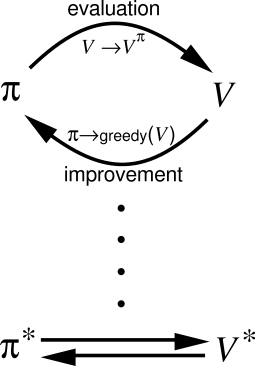
\includegraphics[width=\textwidth]{img/gpi00.png}
	\end{minipage}
	\begin{minipage}[b]{0.55\textwidth}
		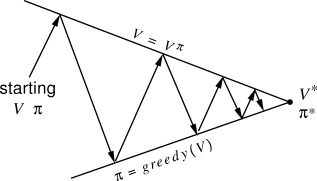
\includegraphics[width=\textwidth]{img/gpi01.png}
	\end{minipage}
	\caption{Generalized policy iteration figure taken from \cite{sutton2018reinforcement}: Value and policy functions interact until they are optimal and thus consistent with other}
	\label{fig:gpi}
\end{figure}

\subsection{Model-Free approach}

As reported in the previous section, having a comprehensive knowledge of the environment is at the foundation of dynamic programming methods. However, this fact is not always accurate in practice, where it is infrequent to have a full understanding of how the world works. In these cases, the agent has to infer the model using its experience, so it has to exploit model-free methods, based on the assumption that there is no prior knowledge about state transitions and rewards.
This section intends to provide a brief description of two model-free approaches to prediction and control: Monte Carlo (MC) methods and Temporal-Difference (TD) ones.

\subsubsection{Monte Carlo learning}

Monte Carlo methods \cite[Chapter 6]{sutton2018reinforcement} can learn from episodes of experience using the simple idea that averaging sample returns provide the value. This lead to the main caveat of these methods: they work only with episodic MDPs because the episode has to terminate before it is possible to calculate any returns.
The total reward accumulated in an episode and the distribution of the visited states is used to calculate the value function while the improvement step is carried out by making the policy greedy concerning the value function.

This approach brings to light the exploration dilemma about how it is possible to guarantee that the algorithm will explore all the states without prior knowledge of the whole environment. $\epsilon$-greedy policies are exploited instead of full greedy policy to solve this problem.
An $\epsilon$-greedy policy is a policy that acts randomly with probability $\epsilon$ and follows the policy learned with probability $(1-\epsilon)$.

Unfortunately, even though Monte Carlo methods are simple to implement and they are unbiased because they do not bootstrap, they require a high number of iteration to converge. Furthermore, they have a wide variance in their value function estimation due to lots of random decisions within an episode.

\subsubsection{Temporal Difference learning}

Temporal Difference (TD) is an approach made combining ideas from both Monte Carlo methods and dynamic programming. TD is a model-free method like MC but uses bootstrapping to make updates as in dynamic programming. The central distinction from MC approaches is that TD methods calculate a temporal error instead of using the total accumulated reward. The temporal error is the difference between the new estimate of the value function and the old one. Furthermore, they calculate this error considering the reward received at the current time step and use it to update the value function: this means that these approaches can work with continuing (non-terminating) environments.
This type of update reduces the variance compared to Monte Carlo one but increases the bias in the estimate of the value function because of bootstrapping.

The fundamental update equation for the value function is shown in \vref{eq:tdlearning}, where \textit{TD error} and \textit{TD target} are in evidence.

 \begin{equation}\label{eq:tdlearning}
	V(s_t) \leftarrow V(s_t) + \alpha \big(\underbrace{\overbrace{r_{t+1} + \gamma V(s_{t+1})}^{\text{TD target}}- V(s_t)}_{\text{TD error} \ (\delta_t)}\big)
\end{equation}

Two TD algorithms for the control problem which are worth quoting because of their extensive use to solve RL problems are \textit{SARSA (State-Action-Reward-State-Action)} and \textit{Q-Learning}.

\textit{SARSA} is an \textit{on-policy} temporal difference algorithm whose first step is to learn an \textit{action-value} function instead of a \textit{state-value} function. This approach leads to focus not to estimate the specific value of each state, but to determine the value of transitions and state-action pairs. \Vref{eq:sarsa} represents the update function of \textit{SARSA}, while \vref{alg:sarsa} summarise its pseudocode.

\begin{equation}\label{eq:sarsa}
Q(s_t, a_t) \leftarrow Q(s_t, a_t) + \alpha [r_{t+1} + \gamma Q(s_{t+1}, a_{t+1}) - Q(s_t, a_t)]
\end{equation}

\begin{figure}
	
	\begin{algorithm}[H]
		\SetAlgoLined
		\DontPrintSemicolon
		\LinesNumbered
		\KwIn{step size $\alpha \in (0,1]$, small $\epsilon > 0$\;}
		Initialise $Q(s,a) \; \forall\; s \in \mathcal{S}, a \in \mathcal{A}$ arbitrarily, except that $Q(\text{terminal}, \cdot) = 0$\;
		\ForEach{episode}{
			Initialise $s_t$ \;
			Choose $a_t$ from $s_t$ using policy derived from $Q$ (e.g.\ $\epsilon$-greedy) 	 \;
			\Repeat{$s_t$ is terminal}{
				Take action $a_t$ $\rightarrow$ obtain $r_{t+1}$ and $s_{t+1}$ \;	
				Choose $a_{t+1}$ from $s_{t+1}$ using policy derived from Q (e.g.\ $\epsilon$-greedy) \;
				$Q(s_t, a_t) \leftarrow Q(s_t, a_t) + \alpha [r_{t+1} + \gamma Q(s_{t+1}, a_{t+1}) - Q(s_t, a_t)]$\;
				$s_t \leftarrow s_{t+1}$ ; $a_t \leftarrow a_{t+1}$
			}
		}
		\caption{SARSA (on-policy TD control) for estimating $Q \approx q_*$}
		\label{alg:sarsa}
	\end{algorithm}
\end{figure}

\textit{Q-learning} \cite{watkins1989learning} is an off-policy TD control algorithm which represents one of the early revolution and advance in reinforcement learning.
The main difference from SARSA is the update rule for the Q-function: it selects the action in respect of an $\epsilon$-greedy policy while the Q-function is refreshed using a greedy policy based on the current Q-function using a max function to select the best action to do in the current state with the current policy.

\Vref{eq:qlearning} represents the update function of \textit{Q-learning}, while \vref{alg:qlearning} summarise its pseudocode.

\begin{equation}\label{eq:qlearning}
Q(s_t, a_t) \leftarrow Q(s_t, a_t) + \alpha [r_{t+1} + \gamma \max_{a}{Q(s_{t+1}, a)} - Q(s_t, a_t)]
\end{equation}

\begin{figure}
	
	\begin{algorithm}[H]
		\SetAlgoLined
		\DontPrintSemicolon
		\LinesNumbered
		\KwIn{step size $\alpha \in (0,1]$, small $\epsilon > 0$\;}
		Initialise $Q(s,a) \; \forall\; s \in \mathcal{S}, a \in \mathcal{A}$ arbitrarily, except that $Q(\text{terminal}, \cdot) = 0$\;
		\ForEach{episode}{
			Initialise $s_t$ \;
			Choose $a_t$ from $s_t$ using policy derived from $Q$ (e.g.\ $\epsilon$-greedy) 	 \;
			\Repeat{$s_t$ is terminal}{
				Take action $a_t$ $\rightarrow$ obtain $r_{t+1}$ and $s_{t+1}$ \;	
				Choose $a_{t+1}$ from $s_{t+1}$ using policy derived from Q (e.g.\ $\epsilon$-greedy) \;
				$Q(s_t, a_t) \leftarrow Q(s_t, a_t) + \alpha [r_{t+1} + \gamma \max_{a}{Q(s_{t+1}, a)} - Q(s_t, a_t)]$\;
				$s_t \leftarrow s_{t+1}$ ; $a_t \leftarrow a_{t+1}$
			}
		}
		\caption{Q-learning (off-policy TD control) for estimating $\pi \approx \pi_*$}
		\label{alg:qlearning}
	\end{algorithm}
\end{figure}

\subsubsection{Temporal Difference Lambda Learning}

As reported previously, Monte Carlo and Temporal Difference learning perform updates in different ways. The first approach exploits the total reward to update the value function, while the second one, on the other hand, works with the reward of the current step. Temporal Difference Lambda, also known as TD($\lambda$) \cite[Chapter 7,12]{sutton2018reinforcement}, represents a combination of these two procedures and it takes into account the results of each time step together with the weighted average of those returns.
The idea of calculating TD target looking n-steps into the future instead of considering only a single step is the baseline of TD($\lambda$). This lead to the formalisation of the $\lambda$-weighted return $G_t^\lambda$

\begin{equation}\label{eq:lambdaG}
G_t^\lambda = (1-\lambda)\sum_{n=1}^{\infty}\lambda^{n-1}G_t^{(n)}
\end{equation}

TD($\lambda$) implementation takes into account an additional variable called eligibility trace $e_t(s_t)$ which indicates how much learning should be carried out for each state for each timestep. It aims to describe how much the agent encountered a specific state recently and \vref{eq:eligibility_trace} describes the updating rule of this value where the $\lambda$ represents the trace-decay parameter.

\begin{equation}\label{eq:eligibility_trace}
e_t(s) = \gamma \lambda e_{t-1}(s) + \mathbbm{1}(s = s_t)
\end{equation}

\subsection{Model-Based approach}


So far, the focus of this section was on methods which have no prior knowledge of the environment, since this thesis grows on model-free foundations.
Despite this point, it is worth to summarise the main concepts behind model-based approaches.
Model-based methods gather information to enable the ability of planning, which can enhance the sample efficiency of the algorithm. 

There are two primary principles to model-based learning. The first one implies to assemble a model starting from prior knowledge and to exploit it to calculate the policy and the value-function, while the second one is to infer the model from the environment by sampling experience.
The central drawback of the first technique is that prior knowledge could be not as accurate as expected, leading to sub-optimal results. Consequently, the preferred way to learn is the second one.

The decisive point behind these approaches is that they are more sample-efficient concerning model-free ones: they require fewer data to learn a policy. On the other hand, the algorithm must learn the policy as well as the model: this translates to two different sources of approximation errors and an increase of computational complexity.

\section{Deep Reinforcement Learning} \label{deepreinflearn}

%\todomacaluso{
%	\begin{itemize}
%		\item Introduction and motivation behind function approximation
%		\item Value-based methods and Policy Gradient methods
%		\item Focus and detailed description of DDPG and SAC
%	\end{itemize}	
%}


The strategies shown so far works smoothly with systems with well-defined states and actions. In this context, it is reasonable to use lookup tables to describe the problem: state-value function V has an entry for each state while in action-value function Q has an entry for each state-action pair.
It is easy to understand how this setting cannot scale up with very large MDPs: problems regarding the availability of memory arise as it becomes difficult to manage the storage of a large number of states and actions. Also, there may be obstacles concerning the slowness of learning the value of each state individually. Furthermore, the tabular form could lead to expensive computation in linear lookup and can not work with continuous action and state space.

Function approximators represent the solution to overwhelm this problem. The underlying intention is to use a vector $\theta = (\theta_1, \theta_2. \dots, \theta_n)^T$ to estimate state-value and action-value function as shown in \vref{eq:fun_appr}, generalise from seen states to unseen states and finally update parameter $\theta$ using MC or TD Learning strategies.

\begin{equation}\label{eq:fun_appr}
\begin{aligned}
V(s, \theta) &\approx V_\pi(s) \\
Q(s, a, \theta) &\approx Q_\pi(s,a)
\end{aligned}	
\end{equation}

In these terms, function approximators can be considered as a mapping from the vector $\theta$ to the value function.
This choice leads to a reduction in the number of parameters to learn and consequently to a system which can generalise better in fewer training samples.

Nowadays, since its widespread use in research, neural networks represent the most intuitive option to take as function approximator: it reduces the training time for high dimensional systems, and it requires less space in memory.
This point represents the bridge between traditional Reinforcement Learning and recent discoveries in the theory of Deep Learning. 
Thanks to the last decade great fervour of Deep Learning, neural networks become the fundamental tool to exploit as function approximator to develop Deep Reinforcement Learning (DRL). This evolution of traditional reinforcement learning accomplished remarkable results. One of the first steps towards Deep RL and general artificial intelligence -- an AI broadly applicable to a different set of various environments -- was done by DeepMind with their pioneering paper \cite{mnih2013playing} and the consequent \cite{mnih2015human}.

This section aims to explain the state-of-the-art and the leading theory behind DRL framework and to define two deep actor-critic algorithms used in the experiments of this thesis: Deep Deterministic Policy Gradient (DDPG) and Soft Actor-Critic (SAC).

\subsection{Fundamentals of Deep Learning}

Deep learning (DL) is an approach to learning based on a function $f: \mathcal{X} \rightarrow \mathcal{Y}$ parametrised with $\theta \in \mathbb{R}^{n_\theta} (n_\theta \in \mathbb{N})$ such that $y = f(x;\theta)$.

The central components of this research field are Neural Networks (NN).
A deep neural network consists of a series of processing layers to which correspond non-linear transformation.
The whole sequence of these alterations directs the learning process through different levels of abstraction \cite{erhan2009visualizing}.
To better understand the nature of a deep neural network, it is convenient to describe a neural network with one fully-connected layer represented by \vref{fig:fullyconnected}. 

\begin{equation}\label{eq:non_linear_transformation}
\begin{gathered}
h = g(w_1 \cdot i + b_1) \\
o = w_2 \cdot h + b_2
\end{gathered}
\end{equation}

The input layer receives as input a column vector of input-features $i$ of size $n \in \mathbb{N}$. Every value of the hidden-layer represented by a vector $h$ of size $m \in \mathbb{N}$ is the result of a transformation of the input values given by \vref{eq:non_linear_transformation} where $w_1$ is a matrix of size $m \times n$ and $b_1$ is a bias term of size $m$. $g$ is a non-linear parametric function called activation function, which represents the core of neural networks. Subsequently, the second and last transformation manipulates the hidden layer $h$ to produce the values of the output layer following \vref{eq:non_linear_transformation} using $w_2$ with size $o \times m$ and $b_2$ with size $o$.  

\begin{figure}
	\centering
	\tikzset{%
		every neuron/.style={
			circle,
			draw,
			minimum size=1cm
		},
		neuron missing/.style={
			draw=none, 
			scale=4,
			text height=0.333cm,
			execute at begin node=\color{black}$\vdots$
		},
	}
	
	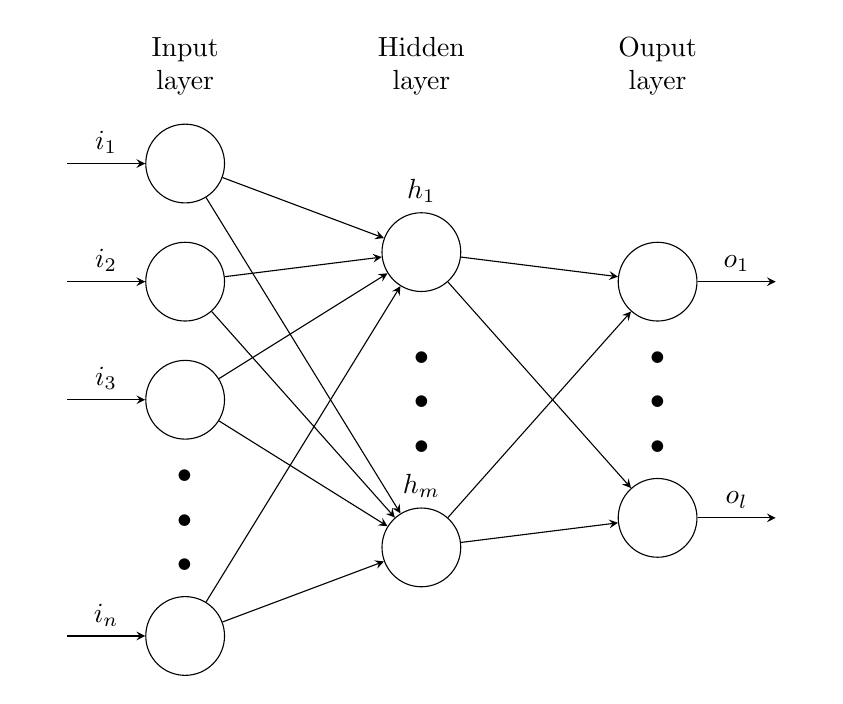
\begin{tikzpicture}[x=1.5cm, y=1.5cm, >=stealth]
	
	\foreach \m/\l [count=\y] in {1,2,3,missing,4}
	\node [every neuron/.try, neuron \m/.try] (input-\m) at (0,2.5-\y) {};
	
	\foreach \m [count=\y] in {1,missing,2}
	\node [every neuron/.try, neuron \m/.try ] (hidden-\m) at (2,2-\y*1.25) {};
	
	\foreach \m [count=\y] in {1,missing,2}
	\node [every neuron/.try, neuron \m/.try ] (output-\m) at (4,1.5-\y) {};
	
	\foreach \l [count=\i] in {1,2,3,n}
	\draw [<-] (input-\i) -- ++(-1,0)
	node [above, midway] {$i_\l$};
	
	\foreach \l [count=\i] in {1,m}
	\node [above] at (hidden-\i.north) {$h_\l$};
	
	\foreach \l [count=\i] in {1,l}
	\draw [->] (output-\i) -- ++(1,0)
	node [above, midway] {$o_\l$};
	
	\foreach \i in {1,...,4}
	\foreach \j in {1,...,2}
	\draw [->] (input-\i) -- (hidden-\j);
	
	\foreach \i in {1,...,2}
	\foreach \j in {1,...,2}
	\draw [->] (hidden-\i) -- (output-\j);
	
	\foreach \l [count=\x from 0] in {Input, Hidden, Ouput}
	\node [align=center, above] at (\x*2,2) {\l \\ layer};
	
	\end{tikzpicture}
	\caption{An example representation of a deep neural network with one fully-connected hidden layer.}
	\label{fig:fullyconnected}
\end{figure}
\Vref{eq:activation} shows the most common activation functions: in general, \textit{ReLu}  achieves better performance over a wide variety of tasks, but usually the selection of the best activation function has to be done starting from all information and requirements of the deep learning model.
\begin{equation}\label{eq:activation}
\begin{aligned}
\text{Sigmoid} \;\rightarrow\;& g(x) = \frac{1}{1+ e^{-x}}\\
\text{Hyperbolic Tangent} \;\rightarrow\;& g(x) = \frac{e^x-e^{-x}}{e^x+e^{-x}}\\
\text{Rectified Linear Unit (ReLu)} \;\rightarrow\;& g(x) = \max(0,x)
\end{aligned}
\end{equation}

$w1$ and $w_2$ in the shown example are the weights of the neural network. The technique used to train these parameters is known as \textit{gradient descent} via the \textit{backpropagation} algorithm. It develops from the concept error and loss function.  The error is the difference between the output of the neural network for a specific input data and the actual value: it is essential to calculate the loss function. One of the most exploited loss function is the Mean-Squared Error (MSE) shown in \vref{eq:backprop}.

\begin{equation}\label{eq:backprop}
\begin{aligned}
L(y, \hat{y}) = (y_\theta - y)^2 \\
J = \frac{1}{n}\sum_{i=1}^{n}L(y_i, f(x_i))
\end{aligned}
\end{equation}

The objective of the gradient descent is to minimise the loss function by modifying the internal parameters of the network using \vref{eq:update} where $\alpha$ is the learning rate.
\begin{equation}\label{eq:update}
\theta \leftarrow \theta -\alpha \nabla_\theta J
\end{equation}

Nowadays, the techniques applied in the majority of research projects is stochastic gradient descent with its various improved extensions and variants, such as ADAM \cite{kingma2014adam} and AdaGrad \cite{duchi2011adaptive}: these extensions manage to improve the convergence of SGD thanks to the introduction of adaptive learning rates.

Another crucial step in deep learning was the introduction of convolutional layers \cite{lecun1995convolutional}. This type of layer revealed is power with images, leading to an increasing interest in image processing field. The parameters of this layer are a set of filters (or kernels) with dimensions smaller than the whole input image: these filters are used to implement a convolution operation over the whole image, and the result serves the input to the next layer in the network. In this context, the network can learn filters that detect specific features in the image such as edges, textures and patterns \cite{erhan2009visualizing}.

\subsection{Approaches to Reinforcement Learning} \label{approaches}


It is possible to explain the main strategies in RL to solve problems using \textit{policy}, \textit{model} and \textit{value function} defined previously.

Every agent has a specific application field which depends on the different approach it supports.
Understanding differences among these approaches is useful to adequately understand what type of algorithm satisfies better the needs of a specific context.

The distinctions presented in this part are just a part of the complete set because this section aims to describe the most crucial distinctions that are useful in the context of the thesis without claiming to be exhaustive.

\subsection{Components of learning}

One of the most crucial aspects of an RL algorithm is the question of whether the agent has access to (or learns) a model of the environment. A model of the environment enables the agent to predict state transitions and rewards.

A method is \textit{model-free} when it does not build a model of the environment. All the actions made by the agent results from direct observation of the current situation in which the agent is. It takes the observation, does computations on them and then select the best action to take.

This last representation is in contrast with \textit{model-based} methods. In this case, the agent tries to build a model of the surrounding environment in order to infer information useful to predict what the next observation or reward would be.

Both groups of methods have strong and weak sides.
Ordinarily, \textit{model-based} methods show their potential in a deterministic environment (e.g. board game with rules). In these contexts, the presence of the model enables the agent to plan by reasoning ahead, to recognise what would result from a specific decision before taking action. The agent can extract all this knowledge and learn an optimal policy to follow. However, this opportunity is not always achievable: the model may be partially or entirely unavailable, and the agent would have to learn the model from its experience. Learning a model is radically complex and may lead to various hurdles to overcome: for instance, the agent can exploit the bias present in the model, producing an agent which is not able to generalise in real environments.

On the other hand, model-free methods tend to be more straightforward to train and tune because it is usually hard to build models of a heterogeneous environment. Furthermore, model-free methods are more popular and have been more extensively developed and tested than model-based methods.


The use of policy or value function as the central part of the method represents another essential distinction between RL algorithms.
The approximation of the policy of the agent is the base of \textit{policy-based} methods. The representation of the policy is usually a probability distribution over available actions. This method points to optimise the behaviour of the agent directly and, because of its on-policy nature, may ask manifold observations from the environment: this fact makes this method not so sample-efficient.
On the opposite side, methods could be \textit{value-based}. In this case, the agent is still involved in finding the optimal behaviour to follow, but indirectly. It is not interested anymore about the probability distribution of actions. Its main objective is to determine the value of all actions available, choosing the best value. The main difference from the policy-based method is that this method can benefit from other sources, such as old policy data or replay buffer.

\subsubsection{Learning settings}

It is possible to classify this method also by different types of policy usage.
An \textit{off-policy} method can use a different source of valuable data for the learning process instead of the direct experience of the current policy. This feature allows the agent to use, for instance, large experience buffers of past episodes. In this context, these buffers are usually randomly sampled in order to make the data closer to being independent and identically distributed (i.i.d): random extraction guarantees this fact.

On the other hand, \textit{on-policy} methods profoundly depend on the training data to be sampled according to the current policy.


\subsection{Taxonomy of Deep RL algorithm}

\begin{figure}
	\centering
	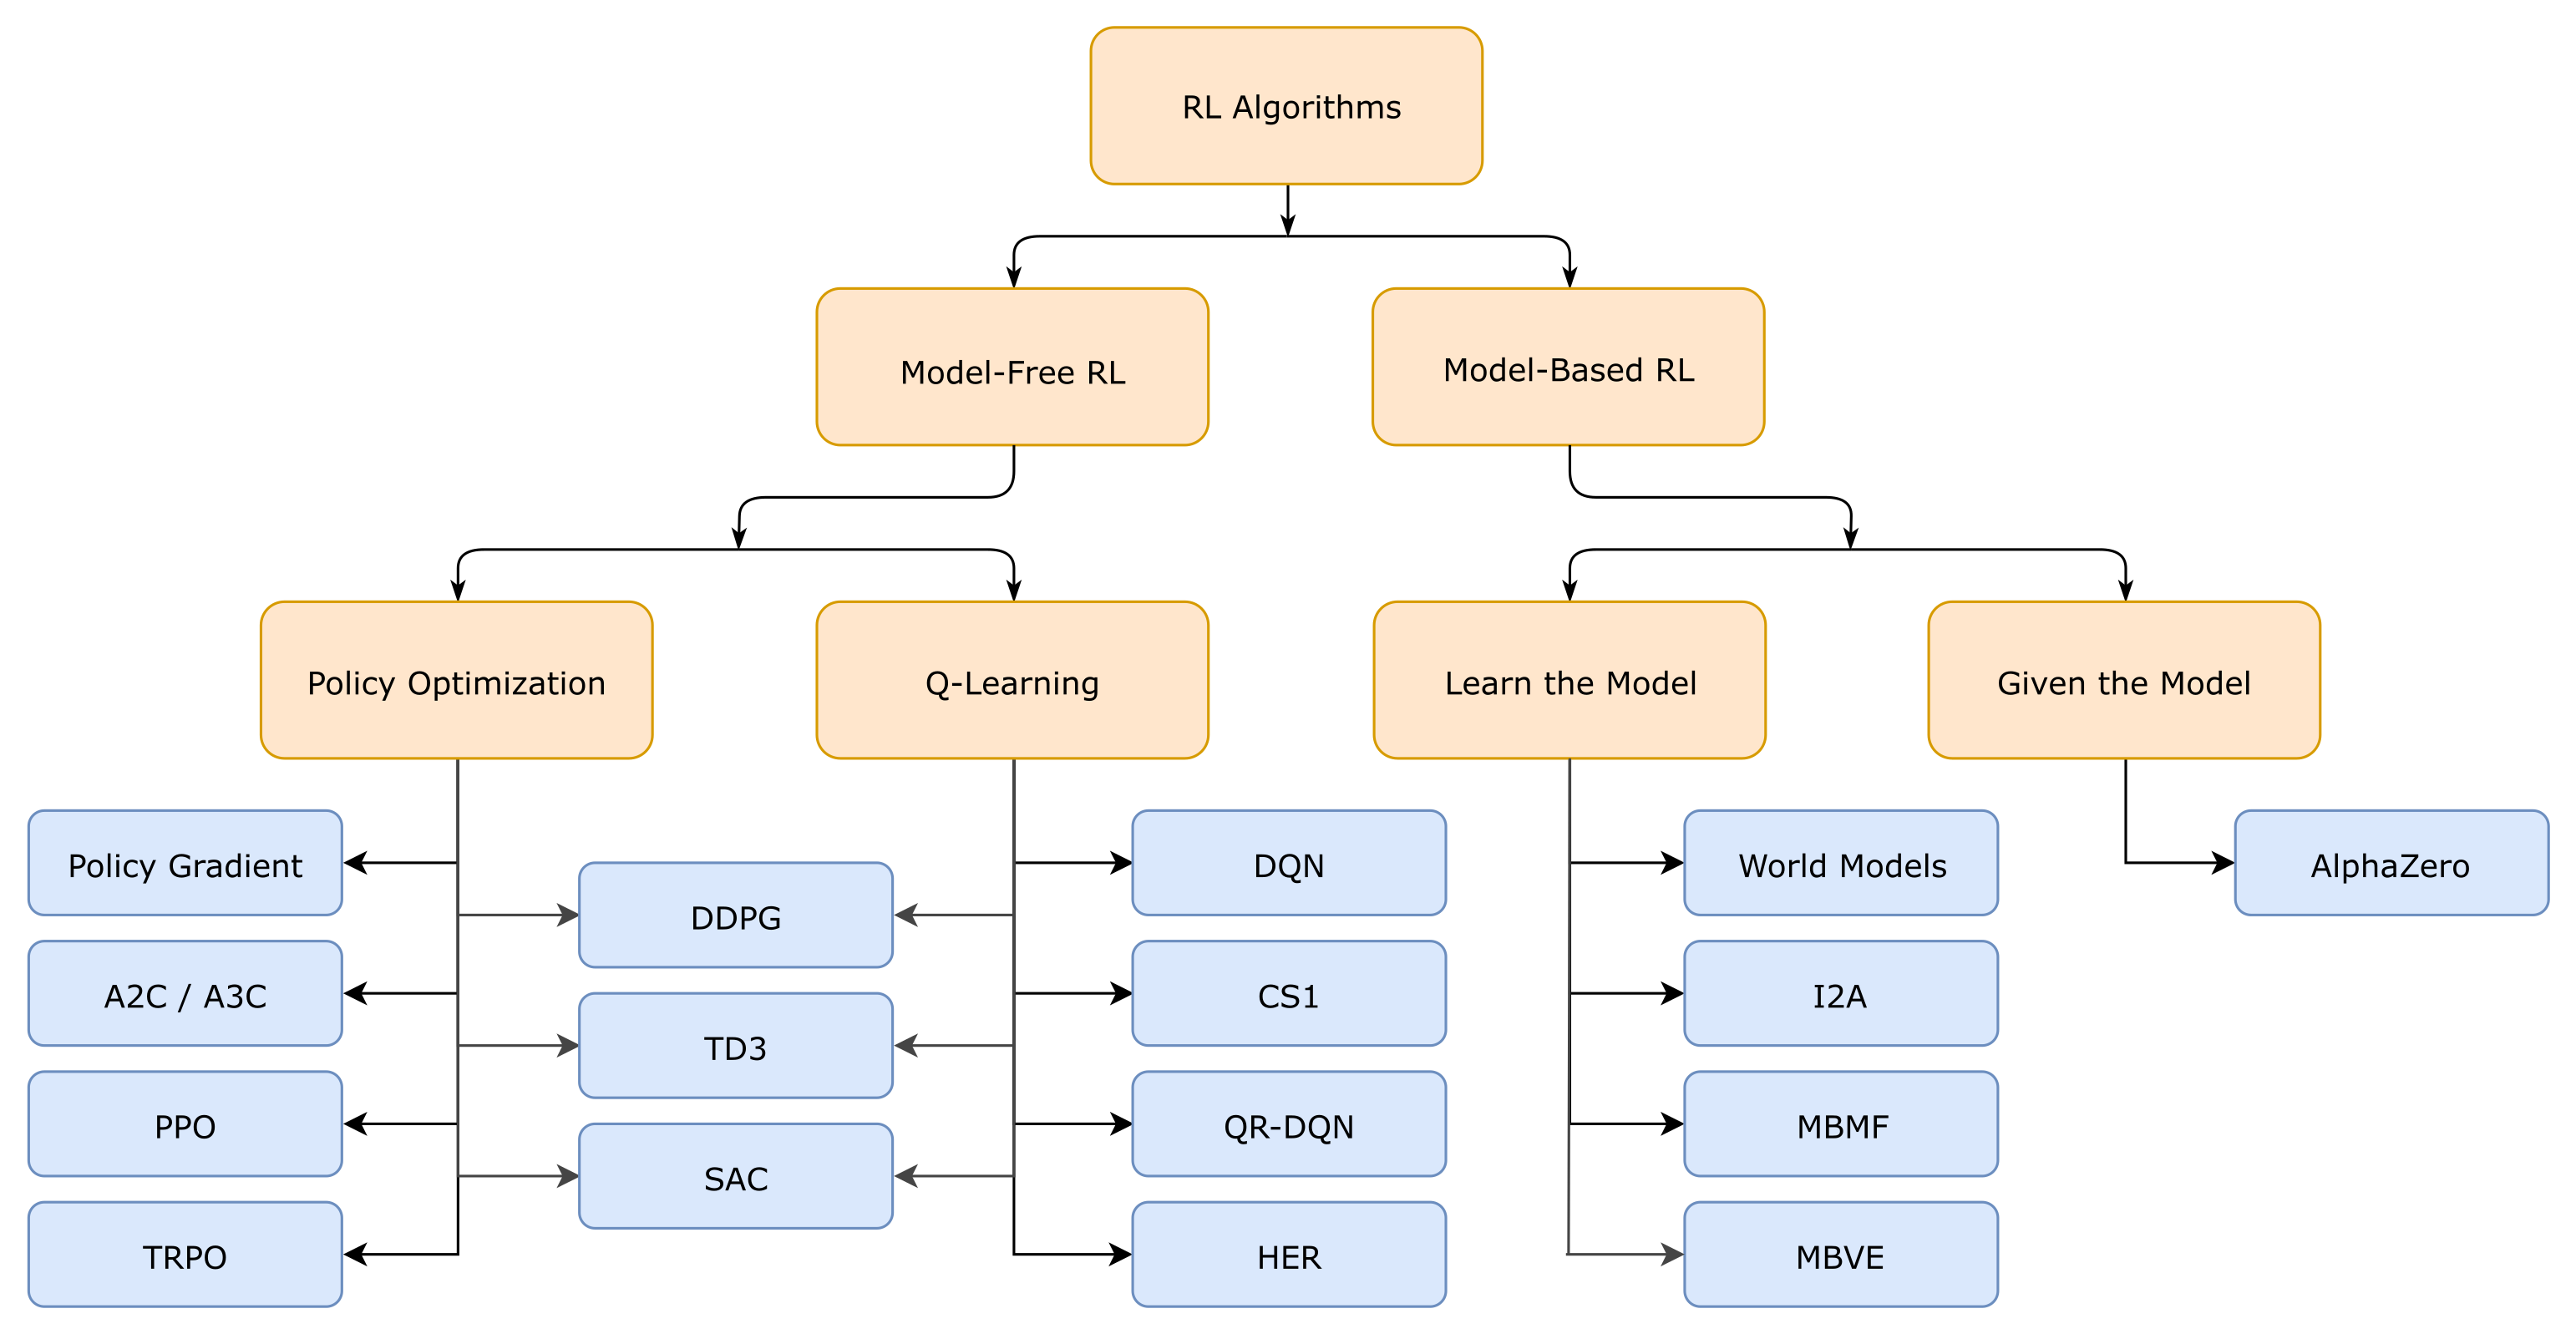
\includegraphics[width=\textwidth]{img/taxonomy.png}
	\caption{A non-exhaustive, but useful taxonomy of algorithms in Deep RL taken from \cite{openai2018spinningup}.}
	\label{fig:taxonomy}
\end{figure}

After the quick overview of the basics of RL terminology and notation provided in the previous section, it is possible to explore more in-depth the universe behind the algorithms of modern DRL. The first significant branching point in \vref{fig:taxonomy} is the distinction between model-free and model-based algorithms, already analysed in \vref{approaches}. 
The second crucial branching point in Deep RL is the question about what to learn. The main components to learn are policies (both stochastic or deterministic), action-value or state-value function and environment models.

Because of the nature of this work, the focus of this section will be on model-free algorithms.

\subsection{Policy Optimization}

As the name suggests, the concept of policy  $\pi_\theta(a|s)$ is central in the techniques of this group. They exploit gradient descent on the performance objective $J(\pi_\theta)$ to update parameters $\theta$ directly. Furthermore, they can indirectly update parameters $\theta$ by maximising local approximation of $J(\pi_\theta)$.

This approach usually works with on-policy optimisation, which implies that every update only uses data gathered with the most recent version of the policy.
In this context, it is also useful to learn an approximator for $V_\phi(s)$ for on-policy value-function $V^\pi(s)$: it is essential to figure out how to update the policy.
Two examples of this type of algorithms are:
\begin{itemize}
	\item \textit{Advantage Actor Critic (A2C)} and \textit{Asynchronous Advantage Actor Critic (A3C)} introduced in \cite{mnih2016asynchronous} are two actor-critic methods which updates parameters directly with gradient descent to maximise performance.
	\item \textit{Proximal Policy Optimisation (PPO)} \cite{schulman2017proximal} increases the performance indirectly by maximising a \textit{surrogate objective} function which tracks how much $J(\pi_\theta)$ changed in the update phase.
\end{itemize}

Policy optimisation methods are principled because they directly optimise the function they want to learn: this fact makes these techniques stable and reliable concerning Q-Learning methods.

\subsection{Q-Learning}

This group of algorithm works learning an approximator $Q_\theta(s,a)$ to infer the optimal action-value function $Q*(s,a)$ using an objective function based upon Bellman equations.
This time, the optimisation presented in this technique is off-policy: this means that the optimisation step is done using all data collected during the whole training, not only with the most recent policy available. In this configuration, the information used for the learning phase could come from exploration decision, not only policy choices.
Thanks to the relation expressed by $a(s) = \operatornamewithlimits{argmax}_a Q_\theta(s,a)$, it is possible to obtain the policy learned so far from the current action-value function.

An example of this technique is Deep Q Network \cite{}, which is one of the most important milestones reached by the research in this field.  \Vref{sec:dqn} provides further information about this algorithm.

Q-Learning is considered less stable than policy optimisation, but they are more sample efficient because they can reuse data more efficiently with respect policy optimisation approaches.

\subsection{Value-Based approaches}

\subsection{Policy Gradient approaches}

\subsection{Deep Deterministic Policy Gradient (DDPG)}

\subsection{Soft-Actor Critic (SAC)}

\section{Related Work}

\todomacaluso{
	\begin{itemize}
		\item Explanation of the state-of-the-art focusing more on Reda's paper, its approach and the related bibliography
\item Increasing interest in Reinforcement Learning applied to real-world situations, in contrast with simulated environments experiments
	\end{itemize}	
}

\section{Summary}







